\section{Wireless Physical Layer}
There are different frequency areas which can be regulated or free.\\
\begin{figure}[!h] 
    \centering 
    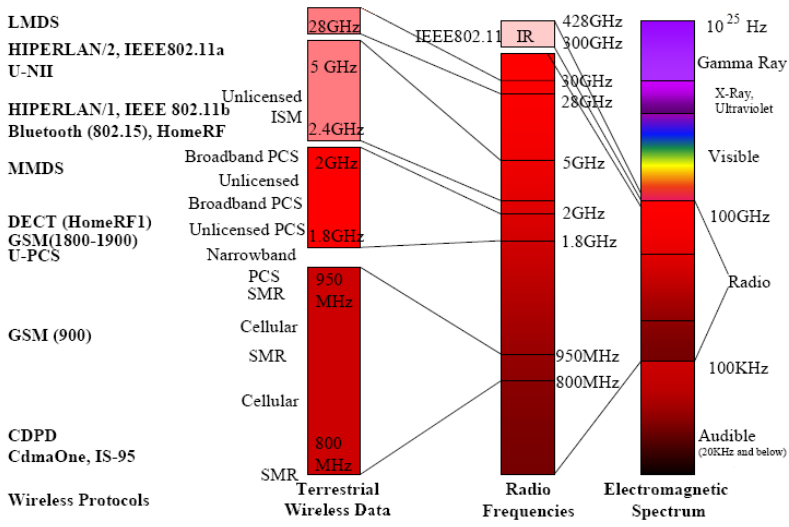
\includegraphics[scale = 0.4]{images/wireless-spectrum.png} 
    \caption{Wireless spectrum}
    \label{wireless-spectrum}
\end{figure}
\begin{figure}[!h] 
    \centering 
    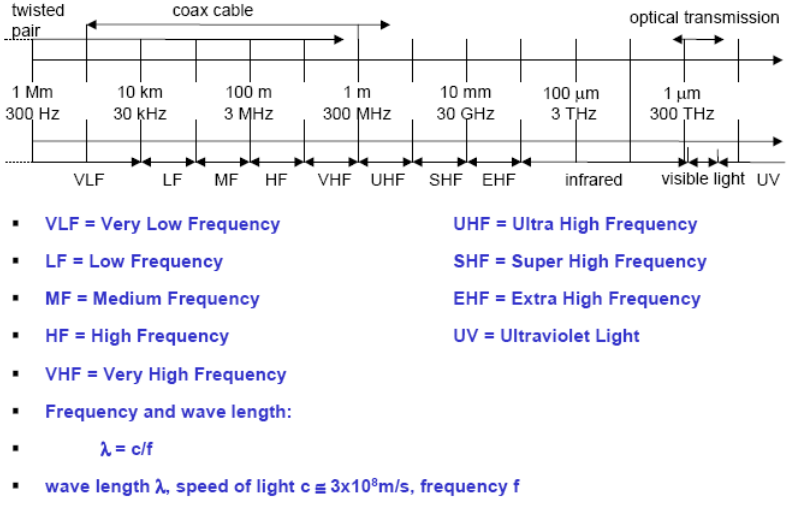
\includegraphics[scale = 0.4]{images/wireless-frequency.png} 
    \caption{Wireless frequency}
    \label{wireless-frequency}
\end{figure}
\newpage
\subsection{Characteristics}
In this section there is some description about the main concepts of wireless\\physical layer\\[0.5cm]
\textbf{Bandwidth} $\rightarrow$ maximum transfer capacity
\begin{itemize}
    \item it can vary between each wireless channel
    \item bits go at the same speed (light physical limit) $\rightarrow$
    gain in encoding/decoding
    \item spectrum can be bigger $\rightarrow$ more space $\Rightarrow$
    more risks (errors, interferences, \dots)
    \item time to accomodate (less time, \dots)
\end{itemize}
\vspace{1em}
\textbf{Coverage}
\begin{itemize}
    \item both isolated $\Rightarrow$ they can't hear each others
    \item if A receives B, but B don't receive A $\Rightarrow$ unidirectional link
    \item if A receives B and viceversa $\Rightarrow$ bidirectional link
    \item Bidirectional links can be:
    \begin{itemize}
        \item[$\rightarrow$] symmetric: A \& B communicate with same speed
        \item[$\rightarrow$] asymmetric: A \& B communicate with different speed
    \end{itemize}
\end{itemize}
\vspace{1em}
\textbf{Technology}\\[0.2cm]
There are different types of technologies used for wireless networks:
\begin{itemize}
    \item Narrowband Radio System
    \begin{itemize}
        \item[$\rightarrow$] used for long distance, LoS needed
        \item[$\rightarrow$] send/receive using a single, licensed, narrowing radio frequency
        \item[$\rightarrow$] cross-talks require coordination/license for each site (low rate)
    \end{itemize}
    \item Spread Spectrum
    it can be of 2 types:
    \begin{itemize}
        \item[$\rightarrow$] Frequency Hopping Spread Spectrum
        \begin{itemize}
            \item it can changes frequency in the way which is known by the\\receiver/transmitter
            \item uninteded receivers may listen to FHSS\footFHSS as impulse noise
            \item lower power/cost/throughput than DSSS\footDSSS
        \end{itemize}
        \item[$\rightarrow$] Direct Sequence Spread Spectrum
        \begin{itemize}
            \item reduntant bit pattern spreded over a large spectrum\\
            $\rightarrow$ long chips can increase the possibility to recover the original bits
            $\Rightarrow$ it may avoid retransmission
            \item uninteded receivers may listen to DSSS\footDSSS as low power wideband noise
            \item high performance, low interferences, good security, more expensive
        \end{itemize}
    \end{itemize}
    \item Infrared
    \begin{itemize}
        \item[$\rightarrow$] it is just below visible light $\Rightarrow$ it can't go beyond obstacles
        \item[$\rightarrow$] LoS is the key (it limitates mobility) $\rightarrow$ short range (indoor, LANs, \dots)
        \item[$\rightarrow$] high data-rate potential
        \item[$\rightarrow$] high bandwidth, easily obstructed, inexpensive
    \end{itemize}
\end{itemize}
\begin{figure}[!h] 
    \centering 
    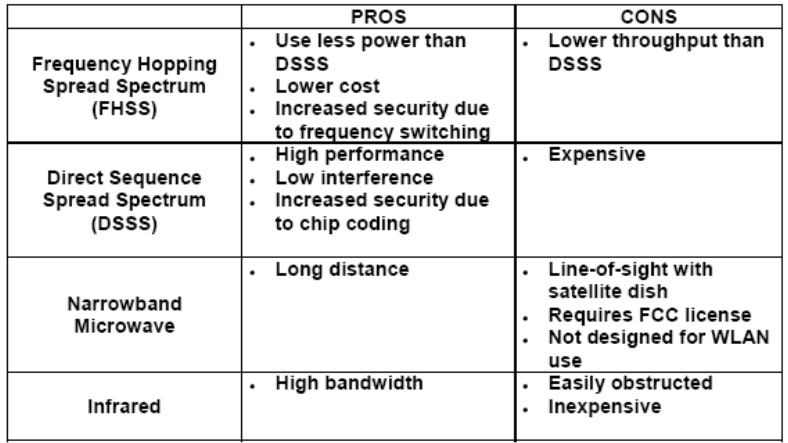
\includegraphics[scale = 0.4]{images/tech-wireless-comparison-physical.png} 
    \caption{Wireless technologies comparison}
    \label{tech-wireless-comparison-physical}
\end{figure}
\textbf{Coverage Areas}\\[0.2cm]
There are different coverege areas:
\begin{itemize}
    \item Wireless Wide/Metropolitan Area Network (WWAN \& WMAN)\\
    It is characterised by the use of:
    \begin{itemize}
        \item[$\rightarrow$] satellites
        \begin{itemize}
            \item GEO $\rightarrow$ 3 of them cover the entire world $\rightarrow$ 500ms Round Trip Time
            \item LEO $\rightarrow$ more mobility, low coverage $\rightarrow$ nodes have to switch\\between them
        \end{itemize}
        \item[$\rightarrow$] cellular/multistructure WLAN
        \begin{itemize}
            \item lots of Access Point all connected to local Mobile terminals
            \item local Mobile terminals connected to internet backbone
        \end{itemize}
    \end{itemize}
    \newpage
    \item Wireless Local Area Network (WLAN)\\[0.2cm]
    It can be of 2 types:
    \begin{itemize}
        \item[$\rightarrow$] Ad-Hoc
        \begin{itemize}
            \item it is a Peer-to-Peer "on the fly" communication
            \item there is no adminstration, no setup, no costs
        \end{itemize}
        \item[$\rightarrow$] Infrastructure
        \begin{itemize}
            \item it is a centralised control unit (Access Point + Local Server)
            \item there is roaming between cells
            \item there is resource sharing and backbone connection
        \end{itemize}
    \end{itemize}
    \item Wireless Personal Area Network (WPAN)
    \begin{itemize}
        \item[$\rightarrow$] it is used for alternative cable connection for in-home/offices
        \item[$\rightarrow$] common protocols are HomeRF, Bluetooth, \dots
    \end{itemize}
\end{itemize}
\vspace{1em}
\textbf{Environment}\\[0.2cm]
There are some challenges to take into account:
\begin{itemize}
    \item capability to maintain needs for apps/services
    \item limited resources such as bandwidth, energy (battery constraints) \dots
    \item device limits (I/O, keyboards, mouse, \dots)
    \item mobility(number of users in the system, \dots)
    \item QoS\footQoS problems, reliability, negotiation\dots
\end{itemize}
\vspace{1em}
\textbf{Multiplexing}
\begin{itemize}
    \item Goal $\rightarrow$ to reach the multiple use of a shared channel\\
    $\Rightarrow$ bandwidth to a large amount of devices
    \item There are multiple options and each one needs to have a guard spaces\\
    $\Rightarrow$ avoid interferences, \dots
    \item Types:
    \begin{itemize}
        \item[$\rightarrow$] Space Multiplexing:
        \begin{itemize}
            \item devices are far away from each other
            \item devices have all the same frequency $\rightarrow$ no interference
            \item guard $\rightarrow$ safety physical space
        \end{itemize}
        \item[$\rightarrow$] Frequency Multiplexing:
        \begin{itemize}
            \item channel's spectrum is divided into smaller bands
            \item host use a single piece for the whole time
            \item guard $\rightarrow$ safety frequency between bands
            \item Pros:
            \begin{itemize}
                \item no dynamic coordination
                \item it works also for analog systems
            \end{itemize}
            \item Cons:
            \begin{itemize}
                \item inflexibility $\rightarrow$ traffic unbalanced $\Rightarrow$ bandwidth waste
            \end{itemize}
        \end{itemize}
        \item[$\rightarrow$] Time Multiplexing:
        \begin{itemize}
            \item one carrier (round-robin) at a time uses the whole bandwidth
            \item guard $\rightarrow$ time between transitions
            \item Pros:
            \begin{itemize}
                \item high throughput for many users
            \end{itemize}
            \item Cons:
            \begin{itemize}
                \item require precise synchronization
            \end{itemize}
        \end{itemize}
        \item[$\rightarrow$] Code Multiplexing:
        \begin{itemize}
            \item how it works:
            \begin{enumerate}
                \item each channel has a unique code
                \item each medium transmits at the same time
                \item messages overlapping
                \item signal combination
                \item receiver decode only what of interest
            \end{enumerate}
            \item Pros:
            \begin{itemize}
                \item no synchronization
                \item more bandwidth
                \item good protection in security/interferences
            \end{itemize}
            \item Cons:
            \begin{itemize}
                \item lower data rates
                \item more expensive $\rightarrow$ it needs to regerate the signal (receiver) 
            \end{itemize}
        \end{itemize}
    \end{itemize}
\end{itemize}
\newpage
\subsection{Wireless vs Wired}
Here there is a comparison between wireless and wired networks.\\
\begin{figure}[!h] 
    \centering 
    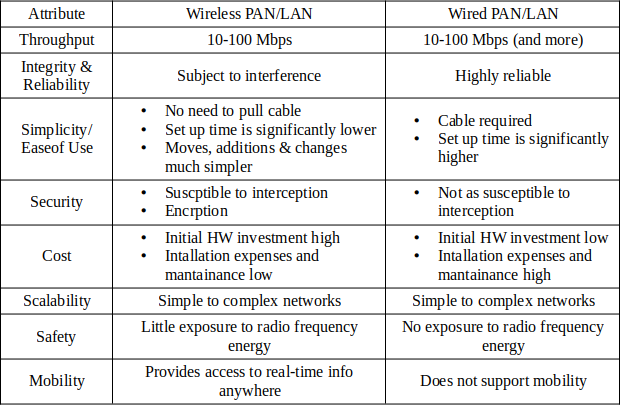
\includegraphics[scale = 0.55]{images/wireless-vs-wired-comparison.png}
    \caption{Wireless vs wired comparison}
    \label{wireless-vs-wired-comparison}
\end{figure}